\section{BERT}
BERT (Bidirectional Encoder Representations from Transformers), 2018 yılında Google tarafından geliştirilmiştir. BERT Base modeli 12 katmana, 786 hidden, 12 self-attention head ve 110M parametreye sahiptir. BERT Large modeli 24 katmana, 1024 hidden, 16 self-attention head ve 340M parametreye sahiptir. "Uncased" modeller hepsi "lower" yani küçük harf metinler ile eğitilmiştir. "Cased" modeller "büyük-küçük" harf korunarak eğitilmiştir. Cümleleri hem soldan sağa hem de sağdan sola olmak üzere çift yönlü olarak değerlendirir. Bu sayede kelimelerin birbirleriyle olan ilişkilerini daha iyi öğreniyor. BERT'in eğitimi için "Masked Language Model (MLM)" ve "Next Sentence Prediction (NSP)" olmak üzere 2 teknik kullanılır.

\begin{figure}[h]
    \centering
    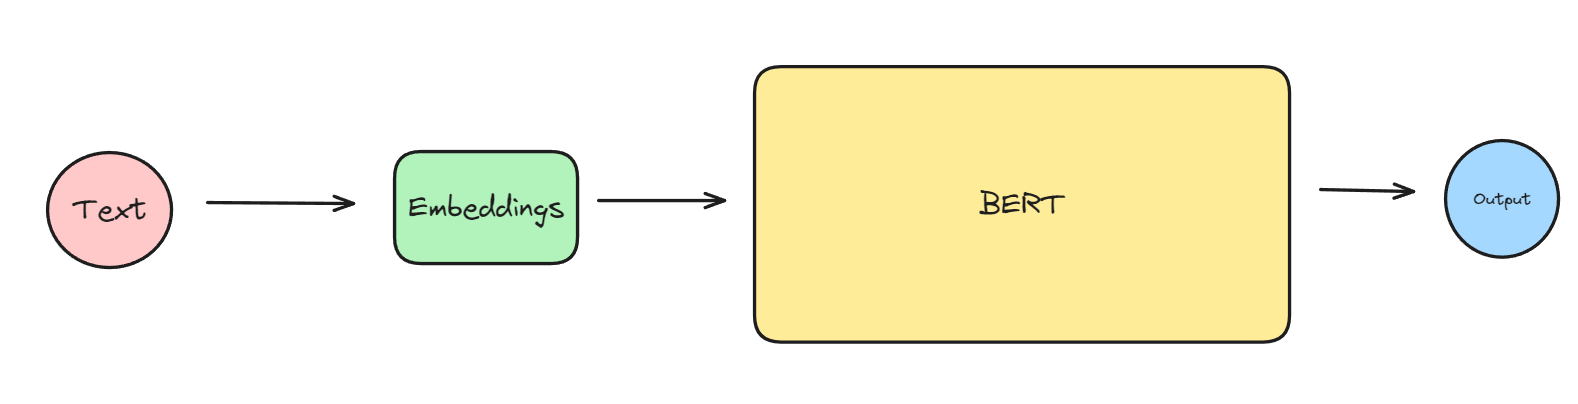
\includegraphics[width=1\textwidth]{images/bert_architecture.png}
    \caption{BERT mimarisi.}
    \label{fig:enter-label}
\end{figure}

\subsection{Masked Language Model (MLM)}
MLM'de, metin içinden \%15'lık kısım rastgele maskelenir. Seçilen kelimelerin \%80'i [MASK] tokeni ile, \%10'u rastgele kelimeler ile kalan \%10 ise değiştirilmeden bırakılıyor. Model maskelenmiş kelimeleri doğru şekilde tahmin etmeye çalışır. Bu, modelin kelimelerin anlamsal ilişkilerini öğrenmesini sağlar. 

\subsection{Next Sentence Prediction (NSP)}
Model rastgele seçilen 2 cümlenin ardışık olup olmadığını tahmin etmeye çalışır. İkili olarak gelen cümlelerin \%50'sinin ikinci cümlesi rastgele değiştirilir. İkili olarak verilen cümlenin ikinci cümlenin ilk cümlenin devamı olup olmadığı tahmin edilir. Bu, metinler arasındaki mantıksal akışı ve bağlantıları anlamasını sağlar. 

\subsection{BERT Tabanlı Modeller}

\subsubsection{RoBERTa (Robustly optimized BERT approach)}
Facebook AI tarafından 2019 yılında geliştirilmiştir. Eğitim verisinde BERT'e göre daha fazla veri kullanılmış ve daha uzun süre eğitilmiştir. Tam maskeleme (full masking) tekniğini kullanmaz. Bunun yerine, her eğitim adımında kelimenin \%15'i gizlenir. Bu, modelin hem bir kelimenin hem de çevresindeki kelimelerin anlamını daha iyi öğrenmesini sağlar. RoBERTa'da BERT'ten farklı olarak NSP (Next Sentence Prediction) kullanılmaz. Araştırmacılar, NSP'den elde edilen faydanın sınırlı olduğunu ve modelin performansını olumsuz etkileyebileceğini düşünmektedir.

\subsubsection{ALBERT (A Lite BERT)}
Amacı BERT'in performansını korurken modelin boyutunu ve hesaplama maliyetini azaltmaktır. BERT'ten daha az parametreye sahiptir. ALBERT, BERT'ten farklı olarak parametrelerin paylaşılmasını kullanır. Bu, modelin daha etkin bir şekilde öğrenmesini sağlar. Parametre paylaşımı, modelin daha az hafıza ve hesaplama kaynağı kullanmasına olanak tanır. Cross-layer parameter sharing, farklı katmanlardaki parametrelerin birbirleriyle paylaşılmasını sağlar. Bu, modelin daha az parametre kullanmasını ve dolayısıyla daha hafif olmasını sağlar. Ayrıca, bu paylaşım modelin daha etkili bir şekilde öğrenmesini sağlayabilir çünkü belirli bir öznitelik türü için kullanılan parametrelerin farklı katmanlarda birbirleriyle paylaşılması, modelin daha kapsamlı bir şekilde bu öznitelikleri öğrenmesine yardımcı olabilir.  All-Shared, dahil olmak üzere kodlayıcı katmanının tüm parametreleri, BERT modelinin tüm kodlayıcı katmanları arasında paylaşılır. Feed Forward, BERT modelinin diğer tüm kodlayıcı katmanları boyunca yalnızca ileri besleme katmanı parametreleri ileri besleme alt katmanlarıyla paylaşılır. Shared Attention, BERT modelinin tüm kodlayıcı katmanlarında yalnızca dikkat kafası katmanı parametreleri dikkat kafası alt katmanlarıyla paylaşılır.  Factorized embedding layer parameterization (Ayrıştırılmış Gömme Katmanı Parametreleştirme), dil modellerinde gömme matrisinin boyutunu azaltmak için kullanılan bir tekniktir. Bu teknik, modelin boyutunu küçültürken hala yeterli bilgi kodlamasını sağlar. Gömme matrisi, bir dil modelindeki kelime dağarcığının boyutu ile birlikte geleneksel olarak büyük olabilir. Örneğin, BERT gibi büyük dil modellerinde, kelime dağarcığı genellikle milyonlarca kelimeyi içerir ve her bir kelime için bir gömme vektörü saklanır. Bu, modelin bellek kullanımını artırır ve hesaplama maliyetini yükseltir. Factorized embedding layer parameterization tekniği, bu gömme matrisinin boyutunu azaltırken hala yeterli bilgi kodlamasını sağlar. Bu teknik, gömme matrisini daha küçük alt matrislere (faktörler) böler. Bu faktörler, orijinal gömme matrisinin daha düşük boyutlu bir yaklaşımıdır.

\subsubsection{DistilBERT}
DistilBERT, BERT'ten daha küçüktür ve daha az parametreye sahiptir. Bu, modelin daha az bellek ve hesaplama gücü gerektirmesini sağlar. DistilBERT, bu boyut azaltmasını başarmak için BERT'in öğrenme sırasında katmanların ve parametrelerin sıkıştırılması tekniğini kullanır. DistilBERT, BERT'ten farklı olarak öğrenme sırasında sıkıştırma (compression) adı verilen bir teknik kullanır. Bu, örneğin, BERT'in çıktılarının daha küçük boyutlu bir görselleştiriciye beslenerek, öğrenci modelin bu çıktıları taklit etmesini sağlar. Bu şekilde, daha az parametre kullanarak aynı performansı elde etmek mümkün olabilir. DistilBERT, öğrenme sırasında bir öğretmen modelin çıktılarından yararlanır. BERT'ten farklı olarak, DistilBERT eğitiminde öğretmen modeli olarak BERT kullanılabilir. Öğrenci model (DistilBERT), öğretmen modelin çıktılarına daha az doğrulukla ulaşarak öğrenir.

\subsubsection{ELECTRA (Efficiently Learning an Encoder that Classifies Token Replacements Accurately)}
ELECTRA (Efficiently Learning an Encoder that Classifies Token Replacements Accurately), Google tarafından geliştirilen bir dil modelidir ve BERT'in (Bidirectional Encoder Representations from Transformers) alternatif bir versiyonudur. ELECTRA'nın temel fikri, BERT'in maskelenmiş dil modellemesi (MLM) yaklaşımına alternatif olarak "tersine maskelenmiş dil modellemesi"ni (Replaced Token Detection, RTD) kullanmasıdır. BERT, eğitim sırasında giriş metinlerindeki bazı kelimeleri rasgele olarak "MASK" işaretiyle değiştirir ve modelin bu maskelenmiş kelimeleri tahmin etmesini ister. ELECTRA ise, giriş metinlerindeki bazı kelimeleri gerçekten değiştirir ve modelin bu değiştirilmiş kelimeleri tespit etmesini ister. Bu, ELECTRA'nın daha az bilgi kaybıyla daha etkili bir şekilde öğrenmesini sağlar. BERT, maskelenmiş dil modellemesi (MLM) yaklaşımı kullanarak jeneratif bir modeldir. Yani, model, maskelenmiş kelimelerin doğru tahminlerini üretmek için olası tüm kelimelerin olasılıklarını hesaplar. ELECTRA ise diskriminatif bir modeldir; yani, model, değiştirilmiş kelimelerin gerçekten değiştirilip değiştirilmediğini belirlemek için bir sınıflandırma görevini gerçekleştirir.

\subsubsection{XLNET}
XLNet, Google tarafından geliştirilen bir dil modelidir ve BERT'in (Bidirectional Encoder Representations from Transformers) bir genişletmesidir. XLNet, transformer mimarisine dayanır ve kendiliğinden doldurma (autoregressive) bir dil modellemesi yaklaşımını benimser. Bu model, daha önceki dil modellerinden farklı olarak çift yönlü bağlamı korurken her kelimenin olası tüm bağlamlarını dikkate alır. BERT, maskelenmiş dil modellemesi (MLM) yaklaşımını kullanırken, XLNet kendiliğinden doldurma modellemesi kullanır. Bu, her kelimenin bağlamını tahmin etmek için önceki ve sonraki kelimelerin kullanıldığı anlamına gelir. Bu, modelin her kelimenin herhangi bir bağlamdaki etkisini daha iyi yakalamasını sağlar. XLNet, permutasyonel dil modellemesi adı verilen bir eğitim görevi kullanır. Bu görevde, giriş metinindeki kelimeler rastgele bir sırayla yeniden düzenlenir ve model, orijinal sırayı tahmin etmek için eğitilir. Bu yaklaşım, modelin bağımsız değişken sıralarının tüm kombinasyonlarını dikkate almasını sağlar, böylece her kelimenin herhangi bir bağlamda etkisinin doğru bir şekilde modellemesine olanak tanır. BERT, çift yönlü bağlamı kodlayan bir dil modeli olarak tanınır, ancak maskelenmiş dil modellemesi (MLM) kullanırken kelimelerin sırasını kaybeder. XLNet, her kelimenin tüm bağlamlarını göz önünde bulundurarak çift yönlü bağlamı korur. Bu, her kelimenin önceki ve sonraki kelimelerle ilişkisini dikkate alırken aynı zamanda tüm belgeyi göz önünde bulundurmasını sağlar. XLNet, hem ileri hem de geri dönüşlü dikkat mekanizmasını kullanarak bağımsız değişken sıralarının tüm kombinasyonlarını dikkate alır. Bu, her bir kelimenin çift yönlü bağlamını daha iyi yakalamasını sağlar.
 
\newpage